\documentclass[10pt, letterpaper]{article}
\usepackage[utf8]{inputenc}
\usepackage{graphicx}
\usepackage{float}
\usepackage{enumerate}
\graphicspath{ {./images/}  }
\usepackage[margin=0.75in]{geometry}

\emergencystretch 5em%
\newcommand{\code}[1]{\texttt{#1}}
\newcommand{\dline}{\par\noindent\rule{\textwidth}{0.2pt}\\}


\title{COMP 421 - Database Systems \\ 
\large Project 3: Application}
\author{Yazdan Zinati\\yazdan.zinati@mail.mcgill.ca\\ 260928077}
\date{\today}

\begin{document}
\maketitle
\newpage
\section{Relational Model}
The relational model has not been modified from Project 2.
\subsection*{Model}
\dline
\code{HealthcareInstitution(\underline{hcId}, phoneNum, name, email, address, website)}
\dline
\code{CommunityClinic(\underline{hcId})}\\
\\
\code{hcId} foreign key referencing \code{HealthcareInstitution}
\dline
\code{BirthingCenter(\underline{hcId})}\\
\\
\code{hcId} foreign key referencing \code{HealthcareInstitution}
\dline
\code{Midwife(\underline{pracId}, name, email, phoneNum, hcId)}\\
\\
\code{hcId} foreign key referencing \code{HealthcareInstitution}\\
\\
note: \code{hcId} has to be \code{NOT NULL} to enforce Midwife's participation constraint in the \code{employs} relationship set.
\dline
\code{Father(\underline{fatherId}, phoneNum, name, email, address, QChcardid, dateOfBirth, profession, bloodType)}
\dline
\code{Mother(\underline{QChcardid}, phoneNum, name, email, adddress, dateOfBirth, profession, bloodType)}
\dline
\code{Couple(\underline{coupleId}, invited, interested, selected, QChcardid, fatherId)}\\
\\
\code{QChcardid} foreign key referencing \code{Mother}\\
\code{fatherId} foreign key referencing \code{Father}\\
\\
note: \code{QChcardid} has to be \code{NOT NULL} to enforce Couple's participation constraint in the \code{constitutesF} relationship set.

\dline
\code{InformationSession(\underline{sessId}, language, date, time, pracId)}\\
\\
\code{pracId} foreign key referencing Midwife\\
\\
note: \code{pracId} has to be \code{NOT NULL} to enforce InformationSession's participation constraint in the \code{hosts} relationship set.
\dline
\code{Invitation(\underline{sessId, coupleId}, attended, registered)}\\

\noindent\code{sessId} foreign key referencing \code{Information Session}\\
\code{coupleId} foreign key referencing \code{Couple}
\dline
\code{Pregnancy(\underline{coupleId, pregNum}, estDueDate, expBirthTimeframe, lastMenstPeriod, isHomeBirth, primaryMidwife, backupMidwife)}\\
\\
\code{coupleId} foreign key referencing \code{Couple}\\
\code{primaryMidwife} foreign key referencing \code{Midwife(pracId)}\\
\code{backupMidwife} foreign key referencing \code{Midwife(pracId)}\\
\\
note: \code{coupleId} is part of the primary key and thus has to be \code{NOT NULL}.
\dline
\code{Appointment(\underline{apptId}, date, time, pregNum, coupleId, pracId)}\\
\\
\code{(pregNum, coupleId)} foreign key referencing \code{Pregnancy}\\
\code{pracId} foreign key referencing \code{Midwife}\\
\\
note: \code{pregNum} and \code{coupleId} has to be \code{NOT NULL} to enforce Appointment's participation constraint in the \code{belongs} relationship set.\\
\\
note: \code{pracId} has to be \code{NOT NULL} to enforce Appointment's participation constraint in the \code{sets up} relationship set.
\dline
\code{Note(\underline{noteId}, timestamp, description, apptId)}\\
\\
\code{apptId} foreign key referencing \code{Appointment}\\
\\
note: \code{apptId} has to be \code{NOT NULL} to enforce Note's participation constraint in the \code{belongs} relationship set.
\dline
\code{Baby(\underline{babyId}, name, gender, timeOfBirth, dateOfBirth, bloodType, pregNum, coupleId)}\\
\\
\code{(pregNum, coupleId)} foreign key referencing \code{Pregnancy}\\
\\
note: \code{pregNum} and \code{coupleId} has to be \code{NOT NULL} to enforce Baby's participation constraint in the \code{born from} relationship set.
\dline
\code{Technician(\underline{techId}, name, phoneNum})
\dline
\code{Test(\underline{testId}, type, datePrescribed, dateSampleTaken, results, dateConducted, lab, techId, pracId, pregNum, coupleId, babyId, QChcardid)}\\
\\
\code{techId} foreign key referencing \code{Technician}\\
\code{pracId} foreign key referencing \code{Midwife}\\
\code{(pregNum, coupleId)} foreign key referencing \code{Pregnancy}\\
\code{babyId} foreign key referencing \code{Baby}\\
\code{QChcardid} foreign key referencing \code{Mother}\\
\\
note: \code{pregNum, coupleId} has to be \code{NOT NULL} to enforce Test's participation constraint in the \code{belongs} relationship set.\\
\\
note: \code{techId} has to be \code{NOT NULL} to enforce Test's participation constraint in the \code{conducts} relationship set.\\
\\
note: \code{pracId} has to be \code{NOT NULL} to enforce Test's participation constraint in the \code{prescribes} relationship set.
\dline
BirthLocation(\underline{hcId, pregNum, coupleId})
\code{hcId} foreign key referencing BirthingCenter\\
\\
\code{(pregNum, coupleId)} foreign key referencing \code{Pregnancy}
\dline
\noindent \textbf{Note: relation names have been pluralized in the db tables to follow convention.}\\
\\
\subsection*{Artificial keys}
\begin{table}[H]
    \begin{center}
        \begin{tabular}{lllll}
            \cline{1-2}
            \multicolumn{1}{|l|}{\textbf{Entity Set}}   & \multicolumn{1}{l|}{\textbf{Artificial key}} &  &  & \\ \cline{1-2}
            \multicolumn{1}{|l|}{HealthcareInstitution} & \multicolumn{1}{l|}{hcId}                    &  &  & \\ \cline{1-2}
            \multicolumn{1}{|l|}{Father}                & \multicolumn{1}{l|}{fatherId}                &  &  & \\ \cline{1-2}
            \multicolumn{1}{|l|}{InformationSession}    & \multicolumn{1}{l|}{sessId}                  &  &  & \\ \cline{1-2}
            \multicolumn{1}{|l|}{Test}                  & \multicolumn{1}{l|}{testId}                  &  &  & \\ \cline{1-2}
            \multicolumn{1}{|l|}{Baby}                  & \multicolumn{1}{l|}{babyId}                  &  &  & \\ \cline{1-2}
            \multicolumn{1}{|l|}{Appointment}           & \multicolumn{1}{l|}{apptId}                  &  &  & \\ \cline{1-2}
            \multicolumn{1}{|l|}{Note}                  & \multicolumn{1}{l|}{noteId}                  &  &  & \\ \cline{1-2}
            \multicolumn{1}{|l|}{Couple}                & \multicolumn{1}{l|}{coupleId}                &  &  & \\ \cline{1-2}
                                                        &                                              &  &  &
        \end{tabular}
    \end{center}
    \caption{Artificial keys created in the relational model}
\end{table}


\section{Application Interaction}

\begin{enumerate}[a.]
    \item
          \textbf{Assume: \code{P0} = 123.}
          \begin{enumerate}[i]
              \item Run a query in the database that shows that midwife with practitioner id \code{P0} does not exist.

                    \begin{figure}[H]
                        \centering
                        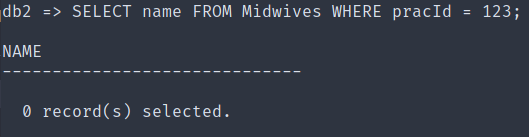
\includegraphics[width=0.5 \textwidth]{a(i)}
                        \caption{a (i)}
                    \end{figure}

              \item Start the application and enter the practitioner id (of the midwife) \code{P0}.
                    \textbf{ii.}
                    \begin{figure}[H]
                        \centering
                        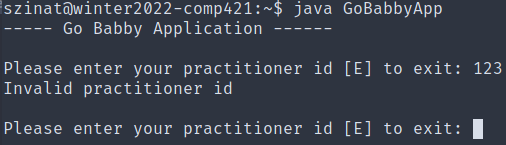
\includegraphics[width=0.5 \textwidth]{a(ii)}
                        \caption{a (ii)}
                    \end{figure}
          \end{enumerate}
    \item \textbf{Assume:
              \begin{itemize}
                  \item mother \code{M1} is named \textit{Victoria Gutierrez}
                  \item mother \code{M2} is named \textit{Corina Solis}
                  \item Appointment date \code {D1} = 2022/03/21.
                  \item Note \code{N1}'s observation is \textit{This is my newest note.}
              \end{itemize}}
          \begin{enumerate}[i]
              \item Run a query in the database that shows that a mother M1 has had at least two pregnancies (can be
                    as part of the same or different couple - does not matter).
                    \begin{figure}[H]
                        \centering
                        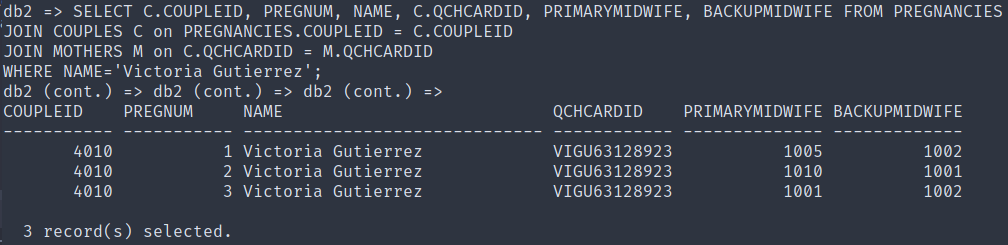
\includegraphics[width=\textwidth]{b(i)}
                        \caption{b (i)}
                    \end{figure}
              \item In the application, enter the practitioner id (of the midwife) \code{P1} (must exist in the database). \\ Assume \code{P1} = 1001.
                    \begin{figure}[H]
                        \centering
                        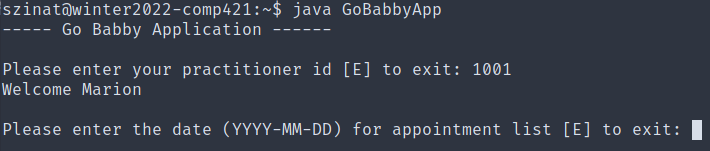
\includegraphics[width=0.8 \textwidth]{b(ii)}
                        \caption{b (ii)}
                    \end{figure}
              \item Enter the date \code {D1}. One of the appointments must be for \code{M1} and another one for \code{M2} , a different
                    expecting mother.
                    \begin{figure}[H]
                        \centering
                        \includegraphics[width=0.8 \textwidth]{b(iii)}
                        \caption{b (iii)}
                    \end{figure}
              \item Choose the appointment number associated with \code{M1}.
                    \begin{figure}[H]
                        \centering
                        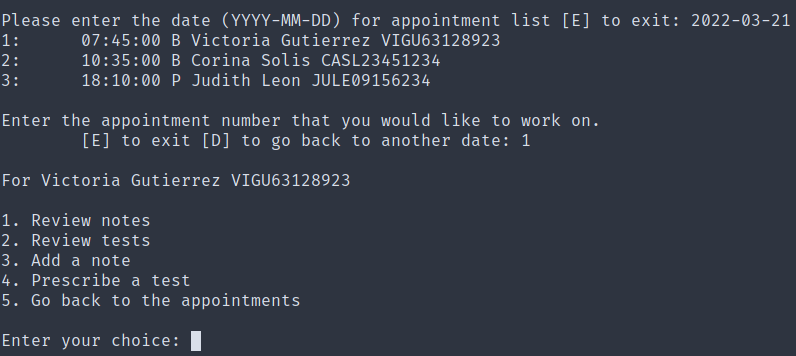
\includegraphics[width=0.8 \textwidth]{b(iv).png}
                        \caption{b (iv)}
                    \end{figure}
              \item Enter 1. (Should show at least two notes).
                    \begin{figure}[H]
                        \centering
                        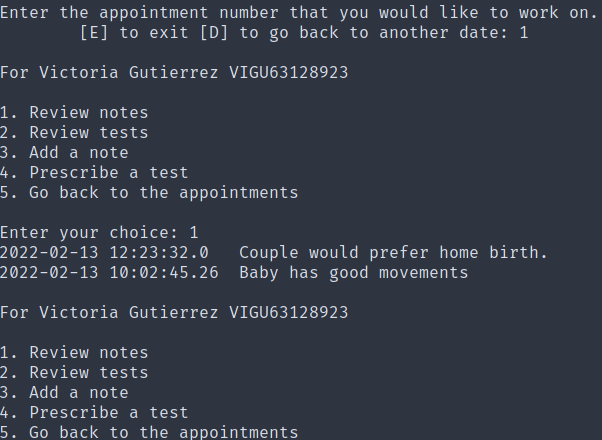
\includegraphics[width=0.8 \textwidth]{b(v)}
                        \caption{b (v)}
                    \end{figure}
              \item Enter 2. (Should show at least two tests).
                    \begin{figure}[H]
                        \centering
                        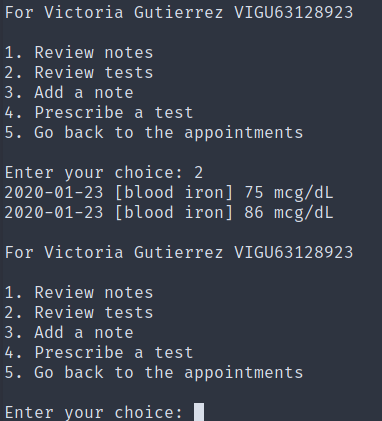
\includegraphics[width=0.5 \textwidth]{b(vi)}
                        \caption{b (vi)}
                    \end{figure}
              \item Enter 3. Add a note \code{N1}.
                    \begin{figure}[H]
                        \centering
                        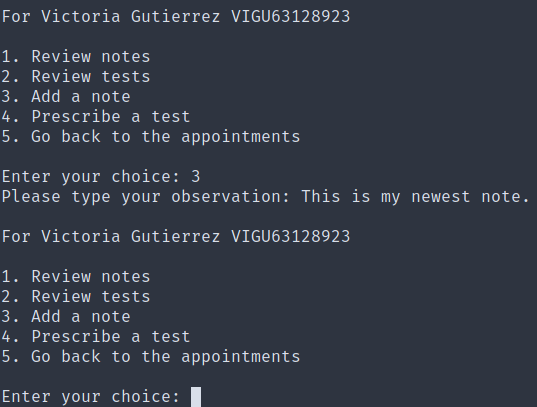
\includegraphics[width=0.6 \textwidth]{b(vii).png}
                        \caption{b (vii)}
                    \end{figure}
              \item Run a query in the database that shows all the notes associated with M1 , include couple information,
                    pregnancy number, etc., as relevant in your model. The actual note text may be truncated to first 50
                    characters or so to reduce clutter.
                    \begin{figure}[H]
                        \centering
                        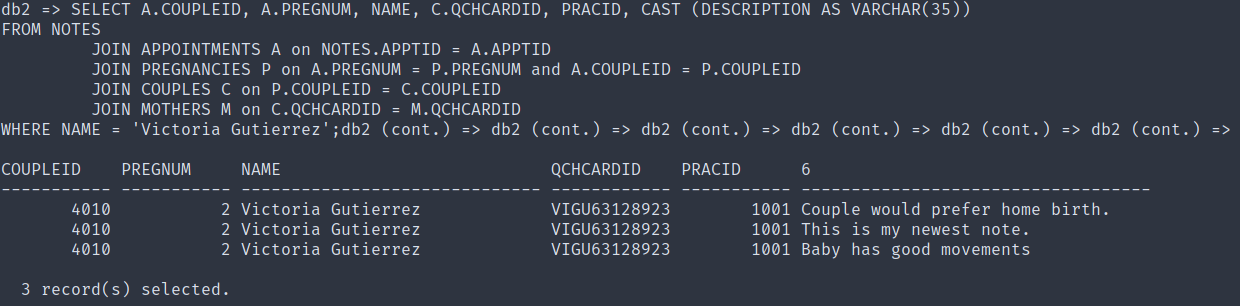
\includegraphics[width=\textwidth]{b(viii).png}
                        \caption{b (viii)}
                    \end{figure}
              \item Enter 1.
                    \begin{figure}[H]
                        \centering
                        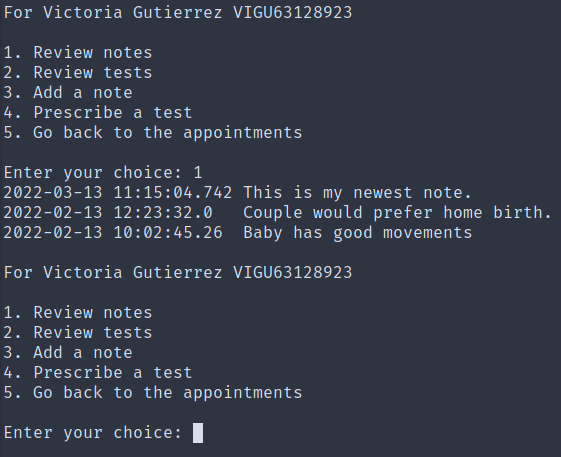
\includegraphics[width=0.6\textwidth]{b(ix)}
                        \caption{b (viii)}
                    \end{figure}
              \item Enter 4. Add a test for trisomy 21.
                    \begin{figure}[H]
                        \centering
                        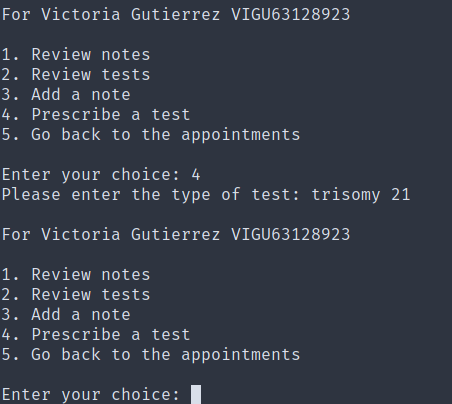
\includegraphics[width=0.6\textwidth]{b(x)}
                        \caption{b (x)}
                    \end{figure}
              \item Run a query in the database that shows all the tests associated with \code{M1} , include couple information,
                    pregnancy number, etc., as relevant in your model. The result attribute of the test maybe truncated
                    to the first 50 characters or so.
                    \begin{figure}[H]
                        \centering
                        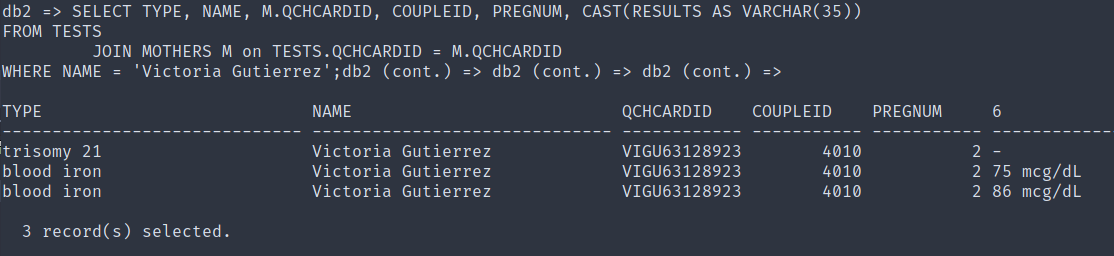
\includegraphics[width=\textwidth]{b(xi)}
                        \caption{b (xi)}
                    \end{figure}
              \item Enter 5
                    (see Figure 15 - c(ii))
          \end{enumerate}
    \item
          \textbf{Assume: mother \code{M2} is named \textit{Corina Solis}}
          \begin{enumerate}[i]
              \item Run a query in the database that shows all the tests associated with \code{M2} , include couple information,
                    pregnancy number, etc., as relevant in your model. The result attribute of the test maybe truncated
                    to the first 50 characters or so.
                    \begin{figure}[H]
                        \centering
                        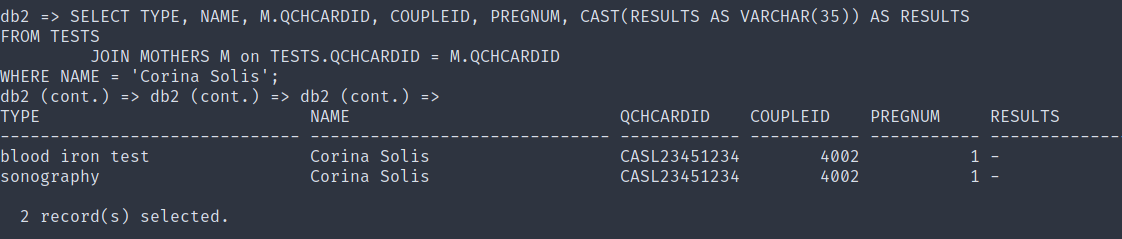
\includegraphics[width=\textwidth]{c(i)}
                        \caption{c (i)}
                    \end{figure}
              \item Choose the appointment associated with mother \code{M2}
                    \begin{figure}[H]
                        \centering
                        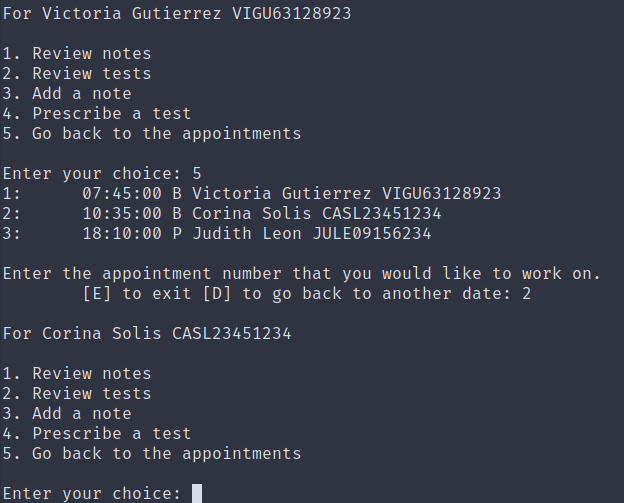
\includegraphics[width=0.5\textwidth]{c(ii).png}
                        \caption{c (ii)}
                    \end{figure}
              \item Enter 1 (to see the relevant notes).
                    \begin{figure}[H]
                        \centering
                        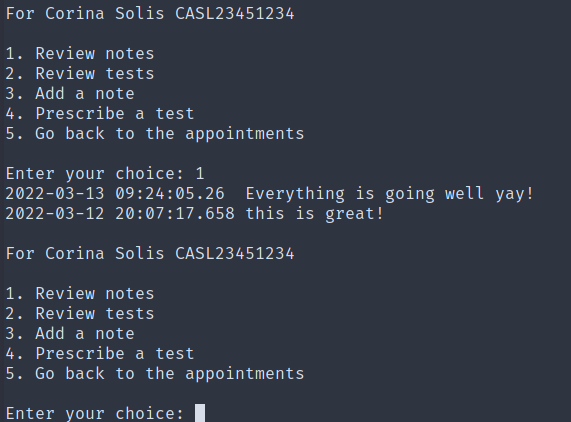
\includegraphics[width=0.5\textwidth]{c(iii).png}
                        \caption{c (iii)}
                    \end{figure}
              \item Enter 4. Add a test prescription for Group B streptococcus (test type).
                    \begin{figure}[H]
                        \centering
                        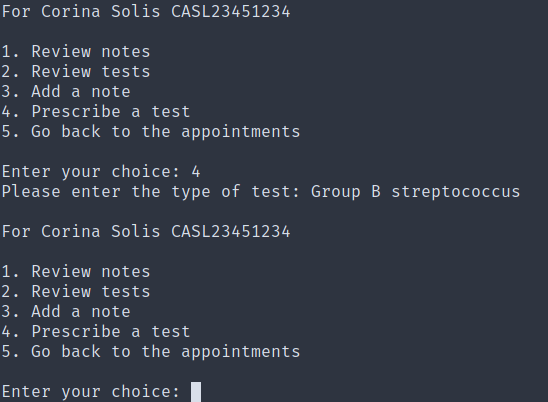
\includegraphics[width=0.5\textwidth]{c (iv).png}
                        \caption{c (iv)}
                    \end{figure}
              \item Run a query in the database that shows all the tests associated with \code{M2} , include couple information,
                    pregnancy number, etc., as relevant in your model. The result attribute of the test maybe truncated
                    to the first 50 characters or so.
                    \begin{figure}[H]
                        \centering
                        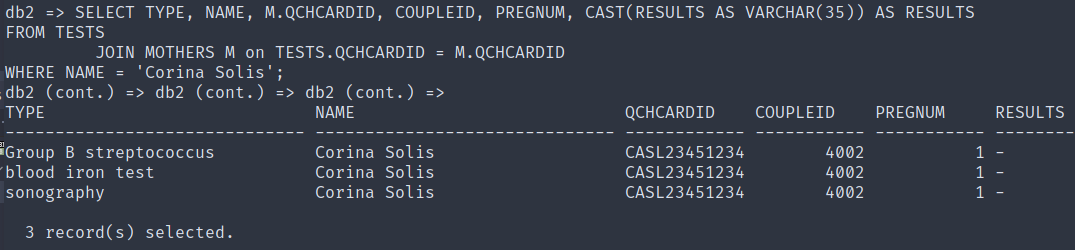
\includegraphics[width=\textwidth]{c (v).png}
                        \caption{c (v)}
                    \end{figure}
          \end{enumerate}
    \item \textbf{Assume appointment date \code{D2} = 2022/05/29}
          \begin{enumerate}[i]
              \item Choose 5, followed by D.
                    \begin{figure}[H]
                        \centering
                        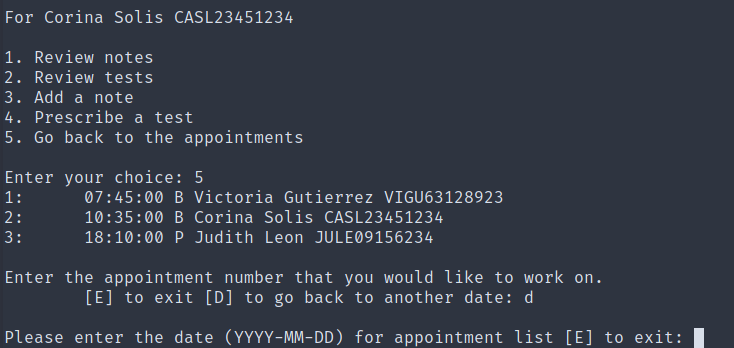
\includegraphics[width=0.7\textwidth]{d(i).png}
                        \caption{d (i)}
                    \end{figure}
              \item Enter a different date D2
                    \begin{figure}[H]
                        \centering
                        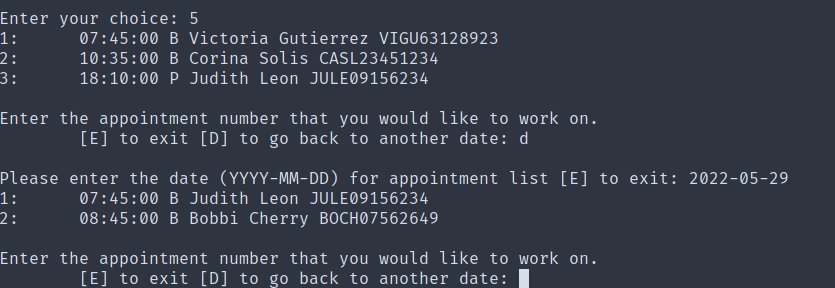
\includegraphics[width=0.8\textwidth]{d(ii).png}
                        \caption{d (ii) and d (iii)}
                    \end{figure}
              \item It should show at least two appointments for mothers M3 , M4 , who are not the same as previous
                    examples.
          \end{enumerate}
\end{enumerate}



\section{Indexing}
Create an index that will help retrieve a mother’s address,
assuming that we only have a phone number to start the search with.
\begin{figure}[H]
    \centering
    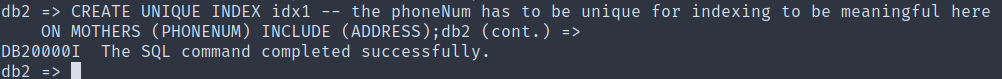
\includegraphics[width=0.8\textwidth]{4}
    \caption{Q4}
\end{figure}

\section{Data Analytics}
\begin{figure}[H]
    \centering
    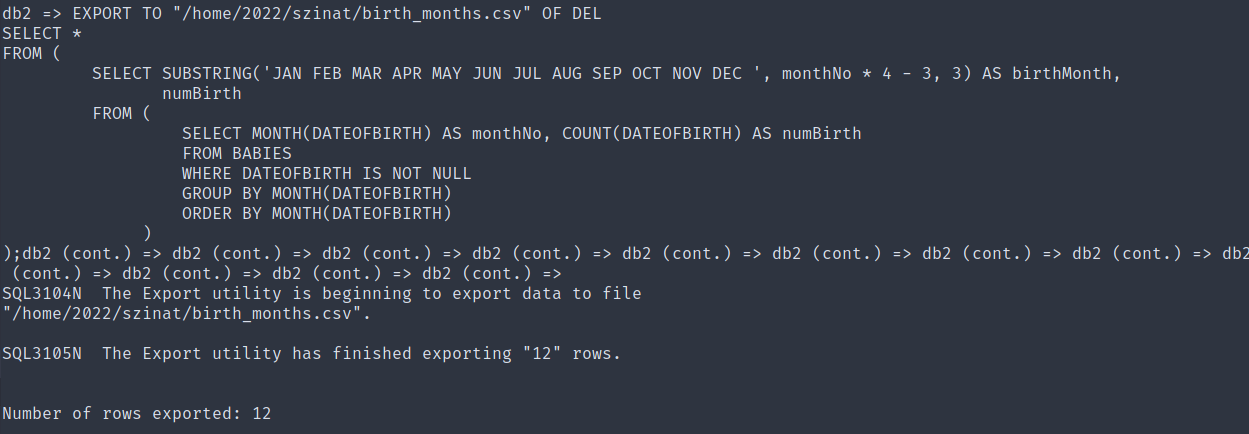
\includegraphics[width=\textwidth]{5}
    \caption{SQL export to export db query into csv file}
\end{figure}

Plot generated using matplotlib.
submitted python code: \code{data\_analytics.py}.
\begin{figure}[H]
    \centering
    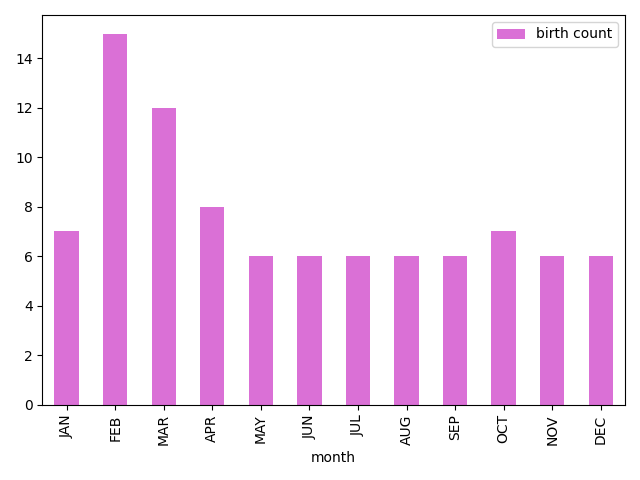
\includegraphics[width=0.7 \textwidth]{pivot_chart.png}
    \caption{Bar plot showing the number of births in each month}
\end{figure}

\end{document}